\chapter{Microscope à feuille de lumière deux photons rotatif}\label{chapIV}

% VolkerComment

% OK
% General remark: Everything that I discussed about the fibers in my first version of the manuscript has to be discussed in your thesis. And you have to extend this and go beyond this and not give less details and less citations.

% VolkerComment
% You have to extend significantly this introduction and link it to the previous chapters. Your aim was to perform the multisensory virtual reality experiments that you described in in Chapter 1 while recording whole brain activity. Two further developments of Geoffrey's setup where necessary
% 1. You needed a system that allows to stimulate the tilt direction.
% 2. You needed a two-photon system to gain high control over the visual stimulus.
% Start with the description to the tilt setup that you developed with Thomas Panier. You can first present it as a one-photon system, talk about the differences in the optical path, the different motor, your control software, the mechanical stability characterization and finish with recordings in one-photon mode. Use the figures of the schematic of the setup and of the one-photon tilt phase maps from the Brighton poster. Then you talk about the transformation of the system into a two-photon setup and the challenge of fiber coupling the two photon laser ... . Here you have to introduce the demands on the fiber coupling properties necessary to develop successfully a 2PRLS. :
% (i) High power transmission and damage threshold
% (ii) low dispersion
% (iii) polarization maintenance
% (iv) low bending loss
% (v) single mode maintenance during bending
%
% [rephrased]
% postural control in virtual environment -> under microscope
% - tilt direction stimulation
%   - differences in optical path
%   - motor
%   - control software
%   - mechanical stability characterization
%   - one photon recordings
%   - brighton phasemaps
% - two-photon system for visual control
%   - fiber coupling
%   - dynamic effects...
% 


% Pour étudier à la fois le système visuel et le système vestibulaire du poisson zèbre, une possibilité est de combiner les deux innovations précédemment citées en un seul microscope : un microscope à feuille de lumière deux photons rotatif. C'est la voie que j'ai explorée, qui a révélé plusieurs défis techniques. Le premier et de guider le laser deux photons vers le module light-sheet en restant stable lors de la rotation du microscope. Le second est de mitiger l'effet de lentille thermique lié à la propagation d'un faisceau haute puissance dans l'eau. Après avoir exploré en détail ces aspects techniques, je montrerai comment le microscope a permis de réaliser l'acquisition du cerveau de la larve sans environnement visuel parasite.


% TODOVolker (à propos de la décroissance de l'intensité dans la direction de propagation)
% Show an image. Is this really an issue. The infrared light interacts less with the tissue compared to the 488nm laser. How do both configurations compare? I do not see uneven fluorescence signal across the fish in two photon recordings.

Pour réaliser l'imagerie du cerveau lors du contrôle postural tel que présenté au chapitre \ref{chapII}, il faut contrôler à la fois l'environnement visuel et l'environnement vestibulaire.
Dans le chapitre \ref{chapIII}, je présente un microscope rotatif capable d'imager le fonctionnement du cerveau lors d'une stimulation vestibulaire réelle, ce qui répond en partie au problème. Dans ce chapitre, je m'intéresse à l'autre partie : comment réaliser l'imagerie tout en contrôlant l'environnement visuel, et cela en même temps qu'une stimulation vestibulaire.

Un microscope à feuille de lumière classique utilise un laser bleu pour stimuler la fluorescence, et cette longueur d'onde réside dans le domaine visible de la larve de poisson zèbre, ce qui peut l'éblouir et perturber son système visuel. Pour cette raison, Ahrens \emph{et al}, pour l'étude de l'OMR, ont utilisé un microscope à deux photons classique \cite{ahrens_brain-wide_2012}. Cela permet d'illuminer dans l'infrarouge, une longueur d'onde invisible pour le poisson. Cependant ils ne bénéficiaient pas des avantages d'un microscope à feuille de lumière et étaient contraints par le balayage point par point à réaliser l'acquisition du cerveau une région après l'autre afin de reconstruire \emph{a prosteriori} l'image du cerveau entier. À peu près en même temps, Truong \emph{et al} publiaient un microscope à feuille de lumière deux photons permettant d'allier les avantages de la microscopie deux photons et de la microscopie à feuille de lumière \cite{truong_deep_2011}.

Plus tard, Vladimirov \emph{et al} \cite{vladimirov_light-sheet_2014} ont montré que l'étude de l'OMR était également possible en microscopie à feuille de lumière un photon, à condition de ne pas éclairer directement l'oeil du poisson. Ils ont utilisé deux feuilles de lumière, l'une éclairant le cerveau par le côté et l'autre par l'avant, entre les deux yeux. Cependant, l'OMR est un réflexe robuste qui ne recourt pas aux fonctions avancées de la vision, et la perturbation due à l'illumination des autres processus visuels n'est pas contrôlée. C'est pourquoi Wolf \emph{et al} ont appliqué la technique mise au point par Truong à l'étude du système visuel de la larve de poisson zèbre \cite{wolf_whole-brain_2015}. Ils ont construit un microscope à feuille de lumière deux photons et réalisé l'acquisition du cerveau entier lors de stimulations visuelles.

Pour étudier le cerveau lors du contrôle postural, il est donc nécessaire de réaliser un microscope rotatif deux photons, ce qui soulève plusieurs enjeux techniques. D'une part, pour guider le laser deux photons vers une plateforme mobile, il faut disposer d'une fibre adaptée (transmission de grandes puissances, faible dispersion, maintient de la polarisation, faible gain de courbure), d'autre part il faut minimiser les effets dus à la propagation d'un faisceau intense dans un fluide mobile. Ce chapitre débute sur les fibres optiques adaptées à la transmission d'un laser deux photons et leur utilisation en microscopie embarquée, et poursuit sur la construction d'un microscope deux photons rotatif fibré.


\section{Effet deux photons}

% TODO améliorer cette section

\subsection{Principe}

L'absorption deux photons est un phénomène non linéaire d'absorption simultanée de deux photons par une molécule ou un atome. Cet effet est proportionnel au carré de l'intensité lumineuse incidente et est lié au caractère anharmonique du dipôle oscillant. Pour cette raison, il est négligeable aux petites énergies mais devient important pour une intensité lumineuse élevée. On peut l'observer en concentrant fortement un faisceau puissant. La concentration peut être à la fois spatiale par focalisation et temporelle par impulsion temporelle.

\subsection{Concentration spatiale}

Un système optique peut concentrer la lumière localement, ce qui produit un point de plus grande intensité, le point focal. Comme l'effet deux photons est proportionnel au carré de l'intensité, la zone concernée est d'autant plus restreinte. Cette propriété est utilisée en microscopie multiphoton pour produire une illumination ponctuelle qui permet le sectionnement optique dans la direction de propagation. En microscopie à feuille de lumière, au contraire, une illumination linéaire est recherchée. La focalisation est donc bien moindre et l'effet deux photons contribue à affiner la zone d'excitation (cf Fig. \ref{2P-intensity-profile}).

\begin{figure}
\centering
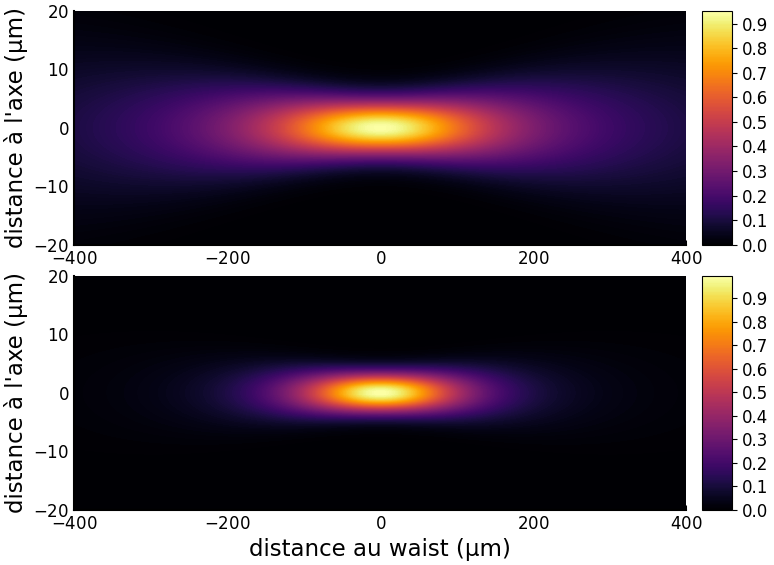
\includegraphics[width=0.8\textwidth]{./files/profile-intensity.png}
\caption{Effet deux-photons en microscpie à feuille de lumière. Comparaison du profil d'intensité (haut) et de son carré (bas). On voit que la zone concernée par l'effet deux photons et restreinte. (paramètres : indice optique 1.33, longueur d'onde 915 nm, waist 6.5 µm)
}
\label{2P-intensity-profile}
\end{figure}

\subsection{Concentration temporelle}

Une autre manière de concentrer la lumière est la concentration temporelle. Dans le cas d'un laser continu, la puissance est répartie sur toute la longueur de propagation du faisceau. En utilisant un laser pulsé, la puissance est concentrée en paquets beaucoup plus courts (cf Fig. \ref{pulsed-laser}). Par exemple, pour des impulsions de 100 fs, malgré la vitesse élevée de la lumière, la longueur de ces paquets est de 30 mm. Si de plus le taux de répétition du laser est de 80 MHz, la puissance moyenne d'une impulsion est 125 fois plus élevée qu'un laser continu de même puissance moyenne (1/(100fs x 80MHz)). L'effet deux photons étant proportionnel au carré de la puissance instantanée, on a intérêt à choisir les impulsions les plus courtes possibles (petit $\tau$) et le taux de répétition le plus faible possible (grand T) pour un laser de puissance moyenne fixée \cite{maioli_fast_2020}. Cette tendance est limitée par les photoperturbations induites, qui deviennent importantes au delà d'une centaines de nanojoules par impulsion. Les conditions optimales en microscopie par fluorescence à nappe laser deux photons sont donc autour de f = 1 MHz, $\tau$ = 100 fs, P = 100 mW.

\begin{figure}
\centering
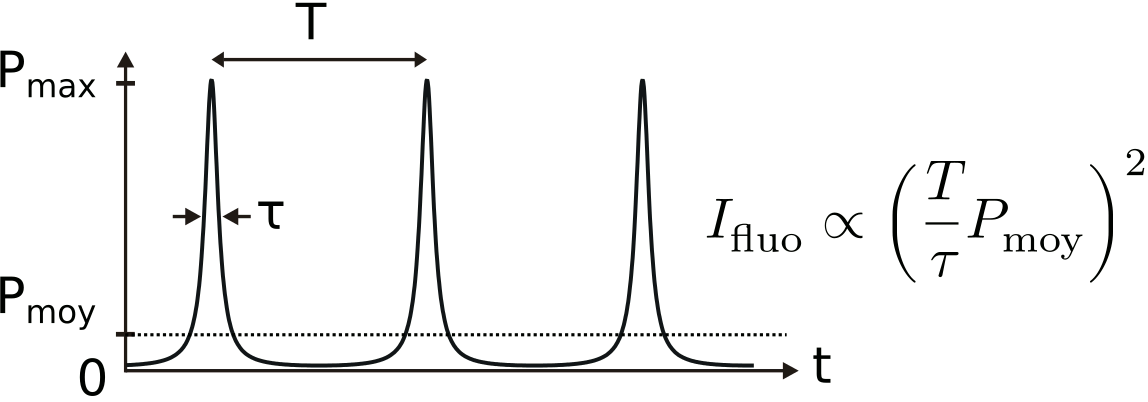
\includegraphics[width=0.8\textwidth]{./files/pulsed_laser.svg.png}
\caption{Profil temporel de puissance d'un laser pulsé. Chaque impulsion a une durée $\tau$, elles sont espacées d'une durée T=1/f. À puissance moyenne constante, plus $\tau$ est petit, et plus T est grand, plus $P_\text{max}$ est grand. L'effet deux photons est proportionnel au carré de $P_\text{max}$.
}
\label{pulsed-laser}
\end{figure}


\section{Fibre optique, principe et état de l'art}


\begin{figure}
\centering
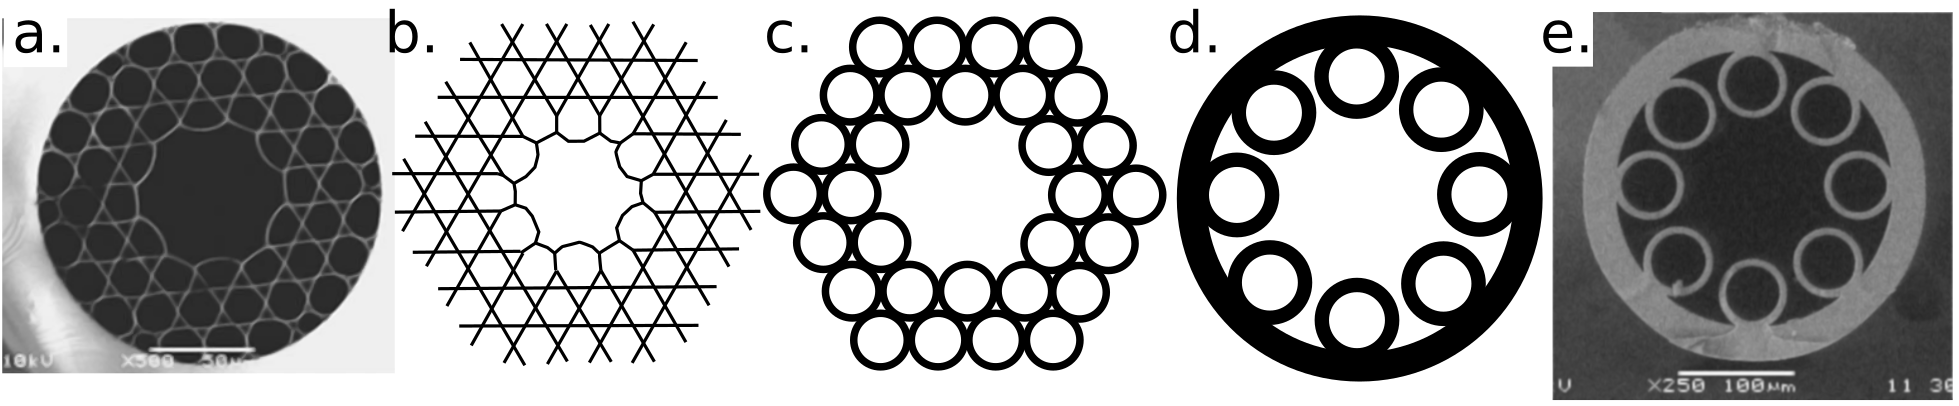
\includegraphics[width=1\textwidth]{./files/fibers.svg.png}
\caption{Illustration de différents types de fibres évoquées.\\
a1. Fibre Kagomé (image extraite de Wang 2011 \cite{wang_low_2011}), schéma du motif en a2.\\
b1. Fibre à réseaux de tube (image extraite de Cregan 1999 \cite{cregan_single-mode_1999}), schéma du réseau tubulaire comme dans Vincetti 2010 \cite{vincetti_waveguiding_2010} en b2.\\
c1. Fibre à courbure négative (image extraite de Yu 2016 \cite{yu_negative_2016}), schéma en c2. Voir également Pryamikov \emph{et al} \cite{pryamikov_demonstration_2011} \\}
\end{figure}

\subsection{Guide d'onde}

Dans un cadre général, un guide d'onde est un objet qui contraint la propagation d'une onde par ses propriétés physiques. Dans le domaine des ondes électromagnétiques aux fréquences radio, par exemple, un tuyau en métal permet de confiner l'onde et de contraindre une propagation unidimensionnelle sur de longues distances \cite{miller_low-loss_1953}, mais également un milieu diélectrique \cite{unger_circular_1957}. On peut lire une revue sur l'histoire de ces découvertes \cite{packard_origin_1984}.
Dans le domaine des fréquences optiques, les guides d'ondes à saut d'indice sont une famille dans laquelle on trouve un grand nombre des fibres optiques utilisée en télécommunications \cite{maurer_glass_1973}. Ces fibres sont constituées d'un coeur de verre entouré d'une gaine d'indice optique plus petit. Dans le cadre de l'optique géométrique, on décrit le guidage par le phénomène de réflexion totale sur le dioptre pour une réfraction en dessus de l'angle limite. Dans le cadre de l'optique ondulatoire, on peut définir les modes propres de la cavité optique. Une fibre est dite monomode si seul le mode fondamental peut se s'y propager.

\subsection{Fibre optique monomode à saut d'indice} % et précompensation de la dispersion

Une fibre optique monomode avec un mode propre quasiment gaussien est adaptée à la transmission d'un faisceau gaussien \cite{ankiewicz_generalized_1992}. C'est le genre de fibre que l'on utilise pour guider le laser d'excitation dans le modèle un photon du microscope à feuille de lumière \cite{migault_whole-brain_2018}. Si l'on tente de transmettre un faisceau pulsé dans ces fibres, on se heurte au phénomène de dispersion \cite{gloge_dispersion_1971} \cite{jurgensen_gaussian_1978}. La largeur spectrale d'un laser pulsé est d'autant plus grande que l'impulsion est courte et la durée de l'impulsion réside dans la synchronicité des différentes fréquences. Dans un milieu dispersif, les différentes longueurs d'onde se propagent à une vitesse différente, ce qui désynchronise les oscillations et élargit le pic. L'effet deux photons étant proportionnel au carré de la puissance instantanée, il est fortement dégradé par l'élargissement du pic. % TODO illustration

Une solution consiste à précompenser cette dispersion via des éléments optiques comme une suite de prismes ou de réseaux de diffraction positionnés en amont de l'injection \cite{fork_negative_1984}. Cette solution permet de réduire la largeur temporelle du pic en sortie de fibre, et donc de conserver l'effet deux photons. On rencontre un autre obstacle pour des impulsions de haute énergie. C'est l'automodulation de phase par effet Kerr \cite{agrawal_nonlinear_2000}. Cet effet est lié aux propriétés non linéaires du milieu traversé, qui change d'indice en fonction de l'intensité lumineuse qui le parcourt. Il en résulte également un élargissement de l'impulsion. Cet effet apparaît pour des puissances moyennes relativement faibles (10 mw \cite{helmchen_miniaturization_2013}), ce qui empêche d'utiliser des impulsions optimalement courtes (<1 ps \cite{helmchen_miniaturization_2013}) avec de telles fibres. Des techniques existent pour précompenser cette distorsion \cite{clark_fiber_2001} \cite{lefort_sub-30-fs_2014}, mais elles sont peu répandues car difficiles à mettre en place \cite{helmchen_miniaturization_2013}. De plus, ces problèmes peuvent être contournés par les fibres à âme vide.

\subsection{Fibre à âme vide}

Les phénomènes de dispersion et de non-linéarité sont dus à l'interaction avec la matière. Pour les contourner, il faut donc que les impulsions à haute énergie se propagent dans le vide. L'effet de réflexion totale sur le dioptre coeur/enveloppe ne peut plus être utilisé, car il faudrait un milieu d'indice plus petit que 1, c'est à dire dans lequel la lumière se propage plus vite que dans le vide, ce qui n'est pas possible. Intéressons-nous au guide d'ondes creux.

\subsubsection{Guide d'onde métallique ou diélectrique}

Une idée pour confiner la lumière dans un guide unidimensionnel est d'utiliser le phénomène de réflexion métallique, comme sur un miroir. En 1964, un article s'intéresse aux guides d'ondes dans le contexte des télécommunications optiques à longue distance \cite{marcatili_hollow_1964}. Les solutions qui semblaient les plus prometteuses à l'époque consistaient soit en une séquence de lentilles et de miroirs, soit en un tuyau métallique ou diélectrique. Le guide d'onde creux circulaire suscite un intérêt pour sa simplicité et sa bonne transmission sur de très longues distances, mais l'article montre que les pertes augmentent très rapidement avec la courbure de la trajectoire.

\subsubsection{Fibres à cristaux photoniques}

Une autre idée consiste à utiliser un phénomène de réflexion par interférences comme le miroir de Bragg. Un tel miroir est constitué d'une succession périodique de couches d'indice différents et permet d'obtenir une réflexion quasi totale à la longueur d'onde du motif. 

\paragraph{Fibres à réseaux de tubes}
On trouve ce genre de réseau pour la première fois en 1999 sous forme de fibre à cristaux photoniques \cite{cregan_single-mode_1999} ou plus tard sous la forme de fibre microstructurées \cite{argyros_hollow-core_2006}. En 2010, Vincetti \emph{et al} montrent par analyse numérique que seule la première couche de tubes joue un rôle important dans les propriétés de ces fibres \cite{vincetti_waveguiding_2010}. Ce qui donne des fibres constituées d'un seul réseau de tube.

\paragraph{Fibres à motif Kagomé}
L'idée du réseau de diffraction a également donné lieu aux fibres à réseau trihexagonal, ou "Kagomé". De telles fibres ont été construites pour la première fois en 2002 sous le nom de fibre à cristaux photoniques. Le gain était alors de l'ordre de 2 dB/m \cite{benabid_stimulated_2002}. En 2011, un gain de 180 dB/km a été obtenu avec de telles fibres \cite{wang_low_2011}.
Cependant, en 2010, Février \emph{et al} montrent par analyse numérique que les propriétés de ces fibres ne reposent pas tant vers le motif périodique que sur la forme du coeur \cite{fevrier_understanding_2010}, ce qui ouvre la voie vers les fibres à coeur hypocycloide. 

% Un des problèmes des fibres à structure géométrique est la sensibilité aux déformations. Puisque le guidage est lié à la géométrie de la fibre, les déformations qui changent cette géométrie altèrent le guidage. Cela peut prendre la forme de perte de transmission, de couplage entre les modes, d'incidence sur la polarisation. Mais cette sensibilité aux déformations dépendant de la géométrie de la fibre, certaines configurations donnent des résultats très satisfaisants.

\subsubsection{Fibres à courbure négative}

Les idées de fibre à réseau de tubes unique et de fibres à coeur hypocycloide se rejoingent dans un même concept : les fibres à courbures négatives. En 2016, Yu et Knight publient une revue sur l'histoire de ces fibres et leurs mécanismes \cite{yu_negative_2016}. Ils commentent entre autres l'atténuation, les bandes de transmission et le gain de courbure. Ces critères rendent cette famille de fibres particulièrement adaptée à notre application. En effet, les larges bandes de transmission permettent de guider plusieurs longueurs d'onde, aussi bien pour l'imagerie un photon que deux photons, la faible atténuation permet de conserver la puissance du laser nécessaire à l'effet deux photons, et le faible gain de courbure permet de conserver une illumination stable pendant la rotation du microscope.

% \cite{belardi_effect_2013}


\subsection{Utilisation des fibres optiques en microscopie embarquée}

% Dans un microscope statique, la source laser peut être guidée jusqu'à l'échantillon par des miroirs, mais dans un microscope mobile il faut soit embarquer la source laser directement sur le microscope, soit la guider de manière flexible quelque soient les mouvements. Dans le cas d'une source laser deux photons très volumineuse, il est impossible de l'embarquer, la solution adoptée est donc une fibre optique adaptée. De telles fibres optiques capables de guider un laser deux photons sont complexes à produire. Avant de nous intéresser aux microscopes à fibre couramment utilisés dans la recherche sur le rongeur, introduisons les caractéristiques d'un guide d'onde. 

Les propriétés de guidage de la lumière d'une fibre optique lui permettent d'alléger considérablement ou de déporter certaines parties des microscopes pour les rendre compatibles avec l'imagerie embarquée. Un microscope est en effet composé d'un axe d'illumination, d'un échantillon, et d'un axe de détection. Les axes peuvent être séparés dans différents bras ou réunis sur une portion du montage optique et sont généralement composés d'éléments optiques rigides passifs tels que des objectifs, miroirs, filtres... Ces différentes parties parfois très volumineuses peuvent être remplacées ou déportées à l'aide de fibres optique. Nous allons voir par la suite plusieurs types de microscopes embarqués utilisant une fibre optique.

\begin{figure}
\centering
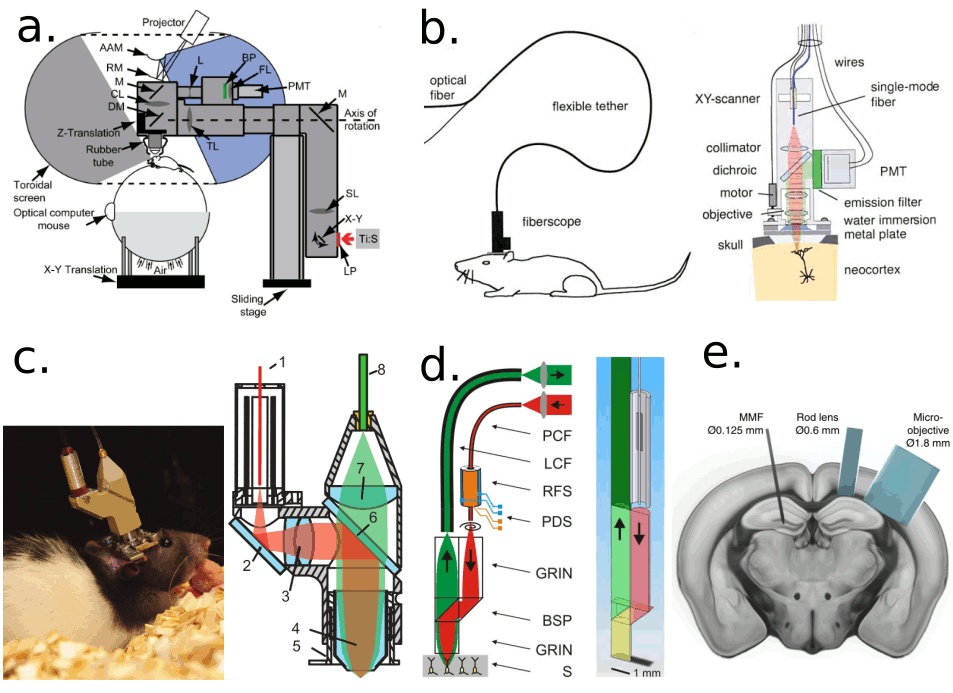
\includegraphics[width=0.9\textwidth]{./files/fiber_functional_imaging.svg.png}
\caption{Différentes techniques de microscopie en imagerie neuronale fonctionnelle chez le rongeur.\\
a. Un microscope deux photons statique réalise l'imagerie du cerveau d'une souris lors d'une expérience en réalité virtuelle \cite{dombeck_functional_2010}.\\
b. Un microscope deux photons est fixé sur la boite cranienne d'un rat. Le laser est guidé à travers une fibre à coeur de verre dont la dispersion est précompensée. L'unité de détection est intégrée au microscope \cite{helmchen_miniature_2001}.\\
c. Un microscope deux photon est fixé sur le crane d'un rat, mais l'unité de détection est externe, la lumière étant collectée par une fibre \cite{sawinski_visually_2009}. \\
d. Un fibroscope deux photons utilise des fibres à gradient d'indice comme lentilles pour réduire l'encombrement. Le laser est guidé au moyen d'une fibre à cristaux photoniques et la lumière est collectée par une fibre à large cœur \cite{engelbrecht_ultra-compact_2008}. \\
e. Un endoscope sans optique permet de réduire considérablement l'encombrement et d'atteindre des régions plus profondes du cerveau, mais nécessite une calibration préalable \cite{turtaev_high-fidelity_2018}.
}
\end{figure}


% Functional imaging in freely moving animals (review)
% Advances in Light Microscopy for Neuroscience (review)

% 1P vs 2P
% Fiber optic in vivo imaging in the mammalian nervous system

\subsubsection{Imagerie sur rongeur à tête fixée}

Une méthode répandue en imagerie cérébrale sur rongeur est de fixer un animal sous un microscope classique immobile. Le cerveau est rendu accessible par une opération chirurgicale pendant laquelle le crane est retiré localement et remplacé par une vitre. Le fait d'immobiliser la tête pendant l'imagerie peut limiter le répertoire comportemental et constituer une gène pour l'animal. Une solution est un système où le rat se positionne volontairement sous le microscope \cite{scott_cellular_2013}, une autre est le système en réalité virtuelle. Dans cette deuxième solution, le rongeur marche sur une boule en polystyrène sur coussins d'air alors qu'un environnement visuel est projeté sur un écran autour de lui \cite{dombeck_functional_2010}. Le microscope est ici entièrement statique et rigide. La réalité virtuelle a également été utilisée avec des enregistrement en électrophysiologie \cite{aronov_engagement_2014}\cite{whitlock_navigating_2014}.


% \subsubsection{Microscope embarqué}
% An implantable and fully integrated complementary metal–oxide semiconductor device for in vivo neural imaging and electrical interfacing with the mouse hippocampus \cite{ng_implantable_2008}

\subsubsection{Déportation de l'illumination}

Une pièce particulièrement volumineuse dans les microscopes multiphotons utilisée pour l'imagerie neuronale est le laser pulsé. En effet, ces systèmes dépendent de beaucoup d'éléments optiques et d'une stabilité thermique et mécanique poussée. Pour construire des microscopes embarqués, il est donc nécessaire de guider le laser depuis la source jusqu'à l'échantillon, ce qui est réalisé à l'aide de fibre optique. Il est possible d'utiliser une fibre optique monomode à cœur de verre \cite{helmchen_miniature_2001} \cite{sawinski_visually_2009} \cite{zong_fast_2017} à condition de précompenser la dispersion pour conserver une impulsion suffisamment courte pour produire l'effet non linéaire recherché, ce qui est réalisé avec une paire de réseaux de diffraction. Une alternative est d'utiliser une fibre à cœur creux \cite{tai_two-photon_2004} \cite{choi_improving_2014} \cite{piyawattanametha_vivo_2009} \cite{klioutchnikov_three-photon_2020}.
La partie de détection est quant à elle également embarquée. On peut avoir un simple photomultiplicateur/photodiode pour l'imagerie par balayage \cite{helmchen_miniature_2001} ou un capteur CMOS pour une imagerie en champ plein \cite{scott_imaging_2018}.

\subsubsection{Déportation de l'illumination et de la détection}

Dans les exemples précédents, le laser est amené par une fibre, mais le capteur est sur place, le signal repartant sous forme de signal électrique. Il est également possible de déporter le système de détection en collectant la lumière par fibre optique. Certains utilisent pour cela une fibre multimode \cite{piyawattanametha_vivo_2009} \cite{sawinski_visually_2009}, d'autres une "fibre plastique" \cite{klioutchnikov_three-photon_2020}, d'autres encore un faisceau de fibres \cite{zong_fast_2017}. Dans ce cas, la lumière collectée est mesurée en sortie de fibre à l'aide d'un système optique adapté sans limite d'encombrement. On peut ainsi utiliser des sytèmes régulés en température ou munis d'une électronique complexe.

\subsubsection{Lentilles à gradient d'indice}

Malgré la déportation de l'illumination et de la détection, les systèmes optiques restent encore assez volumineux du fait des composants utilisés et des éléments mécanique nécessaires. Une possibilité pour pousser la miniaturisation encore plus loin est d'utiliser des fibres à gradient d'indice (\emph{GRIN lens, GRadient INdex lens}). Ces fibres sont constituées d'un milieu à gradient d'indice qui leur donne des propriétés similaires à des lentilles mais sont plus fines et ne nécessitent pas d'éléments mécaniques. Cela permet d'obtenir des microscopes ultra-compacts portables et de poids très réduit \cite{flusberg_vivo_2005}\cite{engelbrecht_ultra-compact_2008}.

\subsubsection{Microendoscopes}

D'autres techniques d'imagerie neuronale se passent même d'optique et sont uniquement consitués d'une fibre insérée dans l'échantillon. On parle alors plutôt de microendoscope. L'idée générale est d'utiliser la même fibre pour éclairer l'échantillon et collecter la lumière. Des éléments actifs peuvent être utilisés pour moduler le front d'onde, et plusieurs techniques reposent sur une phase de calibration préalable \cite{papadopoulos_high-resolution_2013}\cite{ohayon_minimally_2018}\cite{turtaev_high-fidelity_2018}. Ces techniques utilisent des fibres optiques multimodes classiques. L'avantage de l'endoscopie est que les tissus sont traversés par la fibre, et pas directement par la lumière, ce qui contourne le phénomène de dispersion. Il existe également des systèmes plus sophistiqués qui combinent plusieurs fibres en une seule de manière à profiter de propriétés différentes pour l'émission et collection de lumière \cite{andresen_two-photon_2013}\cite{kudlinski_double_2020}\cite{lombardini_high-resolution_2018}.

\section{Caractérisation et utilisation de fibres à âme vide}

Nous avons vu dans la partie précédente qu'une fibre optique permet de guider la lumière, que ce soit pour éclairer l'échantillon ou collecter le signal. Les fibres de verre conviennent bien aux applications classiques, mais posent des problèmes d'interaction lumière-matière lors de la transmission d'impulsions à haute énergie pour la microscopie multiphoton et nécessitent une précompensation de la dispersion. Les fibres à âme vide permettent de contourner ces problèmes et ont déjà été largement utilisées dans des microscopes embarqués sur rongeur \cite{tai_two-photon_2004} \cite{flusberg_vivo_2005} \cite{engelbrecht_ultra-compact_2008} \cite{piyawattanametha_vivo_2009} \cite{choi_improving_2014} \cite{klioutchnikov_three-photon_2020}. C'est donc vers celles-ci que nous nous sommes tournés. Aucune fibre optique répondant à nos besoins n'étant disponible commercialement, nous nous sommes tournés vers l'entreprise \href{http://www.glophotonics.fr/}{Glophotonics} et avons testé plusieurs modèles.

\subsection{Comparaison de fibres}

% OK TODOVolker (GLO all fibers)
% In collaboration with GLO we tested several different fiber types. Go through all of them ! Show the image of the cross section of this fiber and give all details of the fiber geometry: core diameter, total diameter, number of cladding tubes, tube wall thickness, cladding tube diameter, NA, mode field diameter (1/e2), curvature parameter (For b definition, see Opt. Exp. 21, no. 23, 28597, 2013)... .

Au début, nous avons utilisé des fibres ayant une bande de transmission uniquement dans l'infrarouge. Ces fibres ont permis de réaliser l'acquisition deux photons de l'activité neuronale lors de stimulation vestibulaire. Ensuite, nous avons cherché à permettre à la fois la transmission d'un laser 1P et 2P, d'où l'utilisation de fibres avec plusieurs bandes de transmission. Parmi ces fibres, nous avons retenu le modèle PMC-C-9005 B2 qui permet une bonne transmission (97\% à 930 nm sur 1,5 m de fibre contre 70\% pour PMC-C-1C-R\&D2). J'utilise ce modèle comme référence par la suite.

\begin{figure}
\centering
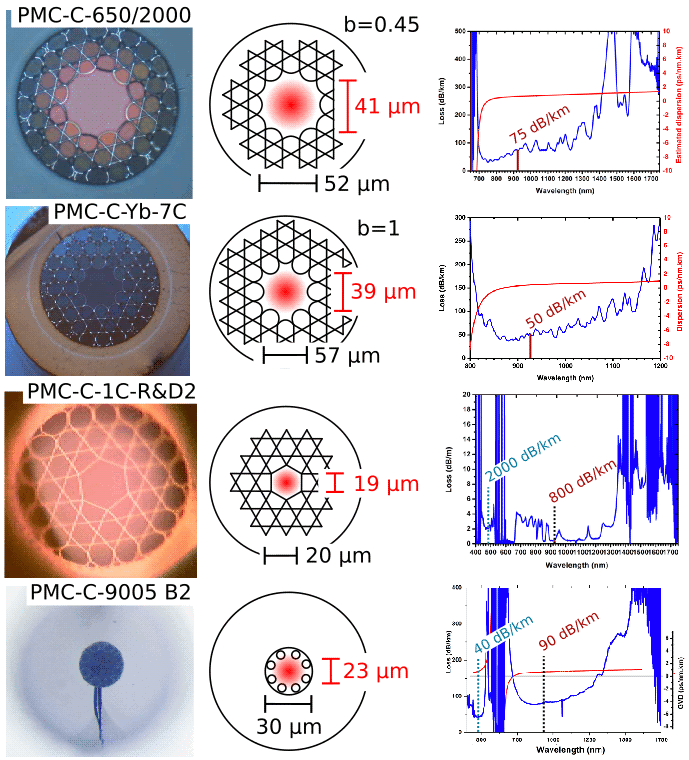
\includegraphics[width=\textwidth]{./files/glofibers.svg.png}
\caption{Comparaison de plusieurs fibres fournies par Glophotonics. Les schémas représentent la largeur du coeur (en noir) et la largeur du mode propre (en rouge). Dans le spectre de transmission, on s'intéresse à la valeur à 930 nm et à 488 nm si possible. La valeur de la dispersion est toujours la même, environ à 1 ps/nm.km. Les trois premières fibres on un motif de Kagomé, alors que la dernière n'est composée que d'une couche de capillaires. Seule la troisième fibre a un coeur hexagonal, les autres on un coeur hypocycloïde. La valeur du paramètre de courbure est notée b, comme défini dans Debord \emph{et al}.  % TODOcite \cite{debord_hypocycloid_2013}
}
\end{figure}


\subsection{Injection d'un laser dans une fibre}

% OK TODOVolker Add a motivation (for 1P)

Une fibre capable de guider à la fois un laser 1P et un laser 2P permettrait de réaliser l'acquisition du cerveau en changeant facilement la longueur d'onde d'excitation. Cela permettrait de mettre en évidence les différences dans l'activité neuronale causées par l'environnement visuel. Je décris ici le processus d'injection dans une fibre et le montage que j'ai mis en place pour passer du laser 1P au laser 2P à l'aide d'un miroir amovible. 

\subsubsection{Principe}

Pour injecter le laser dans la fibre, il faut aligner tous les éléments dans l'axe optique et régler finement les degrés de liberté en translation et en rotation. De plus, comme on souhaite un couplage monomode, il faut faire coincider le mode laser d'entrée de fibre avec le mode propre de la fibre. Le laser ayant un largeur initiale de D, il faut le ramener à une largeur de fibre $w$ (23 µm ± 1 µm d'après la documentation). Pour cela, il faut utiliser une lentille de focale f et satisfaire l'équation suivante :

$$
f = D\frac{\pi w}{4\lambda}
$$

\begin{figure}
\centering
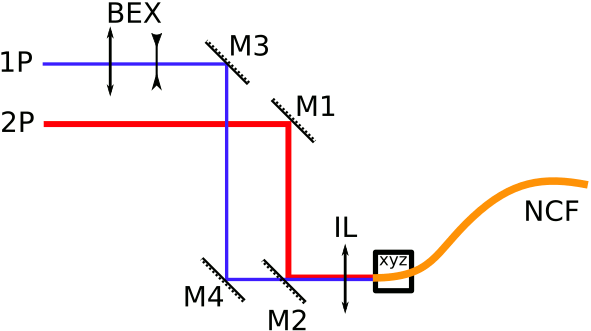
\includegraphics[width=0.8\textwidth]{./files/injection.svg.png}
\caption{schéma de l'injection à deux lasers dans la fibre. Le miroir M2 est amovible et permet de basculer entre l'injection 1P et 2P. (BEX = \emph{Beam Expander}, IL = \emph{Injection Lens}, NCF = \emph{Negative Curvature Fiber})
\\ Pour la première étape, on injecte un laser visible par l'autre extrémité de la fibre et l'on joue sur les miroirs M1 et M2 pour pointer vers la sortie du laser 2P.
\label{FIGinjection}}
\end{figure}

\subsubsection{Injection 2P}

Le laser "Mai-Tai" que j'ai utilisé délivre un faisceau quasiment gaussien (M²<1.1) et son waist ($w_0$) est large d'environ 1 mm. Ces valeurs sont données par la documentation pour une utilisation à 800 nm, mais elles peuvent évoluer légèrement en accordant la longueur d'onde de fonctionnement. La largeur d'un faisceau gaussien au long de sa propagation ($z$) est définie par :

$$
w(z) = w_0 \, \sqrt{ 1+ {\left( \frac{z}{z_\mathrm{R}} \right)}^2 } \qquad \text{avec} \qquad
z_\mathrm{R} = \frac{\pi w_0^2 }{\lambda}
$$

Le diamètre du laser est donc d'environ 2 mm après un mètre de propagation. En prenant D = 2 mm, $\omega$ = 23 µm, et à $\lambda$ = 915 nm, on trouve donc f = 40 mm, c'est pourquoi j'ai utilisé une lentille de focale 40 mm (référence Thorlabs AC254-040-B-ML). Cette lentille dispose également d'un traitement de surface pour optimiser la transmission dans l'infrarouge.

% OK TODOVolker (ref + fig)
% ref to figure
% show a photo of this configuration and explain the alignment procedure with a schema
% Give the damaging threshold of the fiber as a reference -> I do not know

J'ai fixé une extrémité de la fibre sur une platine de translation xyz à 40 mm de la lentille (Fig. \ref{FIGinjection}). Pour faciliter l'alignement, j'ai tout d'abord injecté un laser visible grâce à un connecteur fibre à fibre dans l'autre extrémité. Cela m'a permis de pré-aligner deux miroirs sur support rotatifs en visant l'orifice du laser parallèlement à l'axe optique. En allumant le laser à faible puissance pour ne pas endommager la fibre, on obtient alors facilement une transmission suffisante pour pouvoir mesurer la puissance en sortie de fibre. À partir de cette étape, il suffit d'optimiser la puissance transmise en jouant sur les réglages. Dans un premier temps, les deux degrés de rotations de chacun des deux miroirs, et dans un deuxième temps, les deux degrés de rotation du second miroir et les trois degrés de translation de la platine. Cette technique permet d'obtenir en un temps raisonnable ($\sim$1h) une transmission optimale ($\sim$96\%).

\subsubsection{Injection combinée 2P + 1P}

Pour injecter un deuxième laser, il faut à nouveau faire coïncider le mode de la fibre avec celui du laser, mais en conservant la même lentille d'injection et sans utiliser la platine de translation. Il faut donc adapter la largeur du faisceau à l'aide d'un télescope ou \emph{beam expander} (BEX). En remplaçant 915 nm par 488 nm, on obtient D = 1 mm. La lentille étant optimisée pour l'infrarouge, sa transmission dans le bleu n'est que de 50\%, mais la puissance du laser bleu est suffisante pour compenser cette perte. Par contre, la fibre n'est pas tout à fait monomode à cette longueur d'onde, et l'on distingue clairement en sortie le mode TEM11 ou les modes TEM10 / TEM01 en fonction de la position de la fibre. La meilleure transmission obtenue est de l'ordre de 50\%, mais cela est suffisant pour l'imagerie statique (fibre immobile).


\subsection{Propriétés}

% TODO introduire

\subsubsection{Dispersion et pré-compensation}

Un paramètre important pour la transmission d'un laser pulsé est la dispersion. C'est celui qui nous force à utiliser des fibre à cœur creux et qui permet de conserver une impulsion aussi courte que possible. Mais la dispersion d'une fibre à cœur creux n'est pas nulle, elle est de l'ordre de 1 ps/nm/km (élargissement temporel / largeur spectrale / distance parcourue) comme on peut le voir sur la courbe. La largeur spectrale d'une impulsion est donnée par

$$
\Delta \lambda_t = \frac{\lambda^2}{c\Delta t}
$$

et vaut donc 28 nm. Pour une impulsion de 100 fs à 915 nm, cela donne un élargissement de l'ordre de 28 fs au bout d'un mètre de propagation dans la fibre, soit une perte de concentration de 30\% et donc une perte d'effet deux photons de 50\%. Heureusement, il est possible de pré-compenser cette dispersion à l'aide d'un système optique placé en amont de la fibre. Le laser "Mai-Tai" est justement accompagné d'un élément "Deepsee" qui permet une telle précompensation réglable de -8 900 à -24 500 fs² d'après la documentation.

% (citation documentation)
% > The amount of dispersion, or GVD compensation, provided for each wavelength depends on the position of the DeepSee motor that moves optical material on a stage within the beam path.

En mesurant la durée de l'impulsion en sortie de fibre à l'aide d'un autocorrélateur, on confirme que la précompensation permet de retrouver une impulsion de 100 fs dans l'échantillon.

\subsubsection{Gain de courbure}

% TODOVolker show the data and give all fiber details (fiber bending loss)
% TODOVolker (kagome bending loss)
% This is true for the hypocycloid fibers but does not apply to my knowledge to the Kagome fiber lattice that you discussed just before. Explain why there is a dependence of the gain on curvature. And explain the waveguidance mechanism in the hypocycloid fibers (anitresonance effect ... )

Les propriétés de transmission de la fibre peuvent varier avec la courbure de celle-ci. La transmission est généralement optimale pour une fibre droite et peut se déteriorer suivant le rayon de courbure avec des pertes mesurées en dB. Une fibre PCNC-FC-K13-001 que je ne présente pas ici donnait des variations de transmission de l'ordre de 20\% pour un rayon de courbure de 5 cm.
Lors d'une expérience, la rotation du microscope engendre des déformations de la fibre, et donc des variations de transmission. L'éclairage incident se retrouve corrélé à la stimulation, ce qui crée un signal parasite. Un signal parasite supérieur à 1\% déteriore trop le rapport signal à bruit et empêche l'analse des données. On cherche donc à caractériser les pertes de transmission liées à la courbure. Pour cela, il suffit de placer un puissance-mètre en sortie de fibre et de faire varier la courbure.

Des modèles numériques \cite{setti_flexible_2013} \cite{yu_negative_2016} \cite{frosz_analytical_2017} suggèrent que le gain évolue de manière inversement proportionelle au carré du rayon de courbure. Cette relation est également observée sur notre fibre.
Les pertes par mètre de fibre courbée restent cependant petites même pour un rayon assez court. Elles valent 0.1 dB ($\sim$2\%) pour un rayon de courbure de 7 cm.

En conditions réelles, ont peut s'arranger pour limiter la courbure. Par exemple, la fibre peut être placée le long d'une tige de rigidité plus élevée

% TODOVolker (fiber curvature real conditions)
% pourqui c'est le pire des cas ? Dans quelle context? I do not understand your argument. What is the range of curvature change in your experimental configuration?

\begin{figure}
\centering
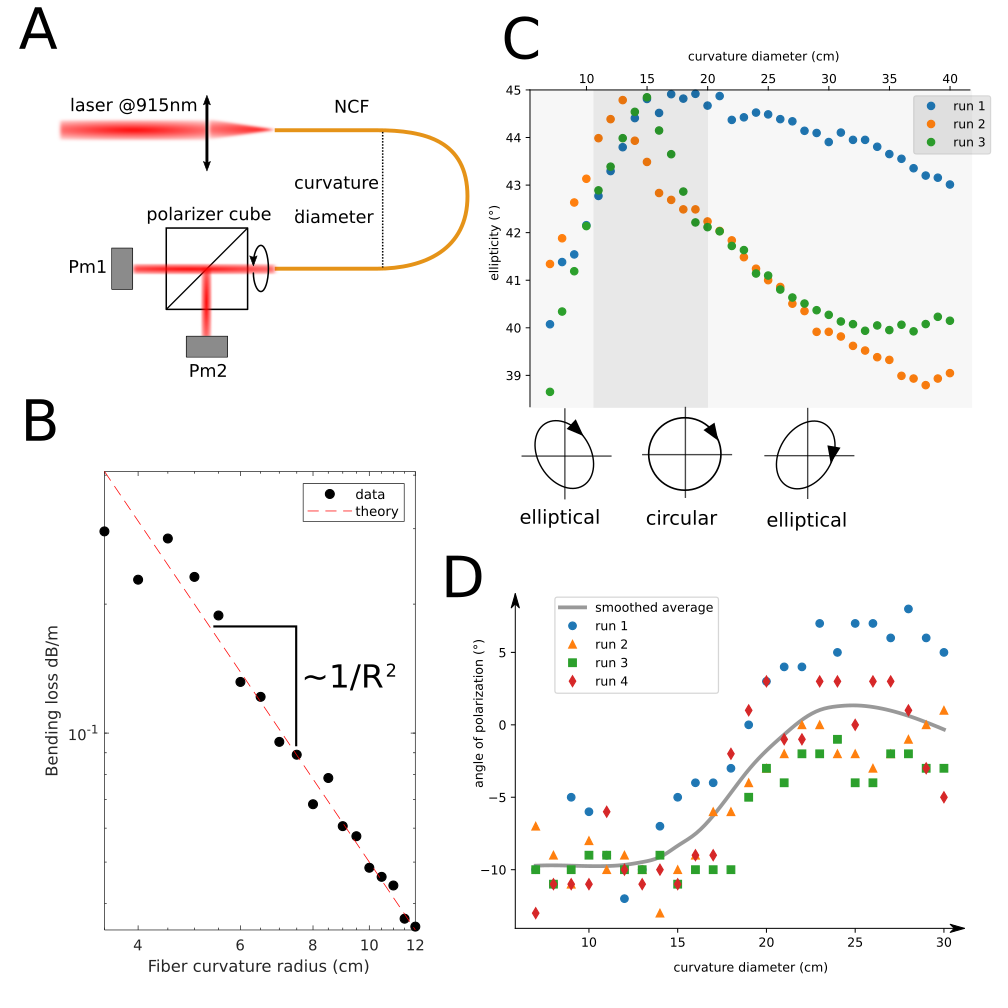
\includegraphics[width=0.8\textwidth]{./files/fiber_bending.png}
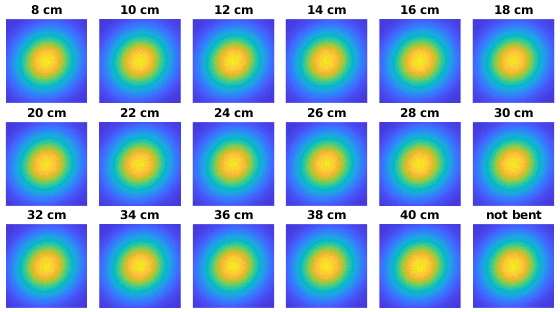
\includegraphics[width=0.6\textwidth]{./files/beam_profile.png}
\caption{Propriétés de la fibre lors d'une courbure.
\\ A. schéma du setup de catactérisation
\\ B. gain en fonction de la courbure
\\ C. ellipticité en fonction de la courbure (quasi circulaire)
\\ D. angle de polarisation en fonction de la courbure (quasi linéaire)
\\ Au dessous figure le profil en sortie de fibre pour différentes courbures. Il n'est pas affecté.}
\end{figure}

\subsubsection{Polarisation}

% TODOVolker (context for polarization -> de Vito)
% You start this paragraph totally out of context. So far you talked about the fiber properties. Here you talk about detected signal in the light sheet configuration. You have to introduce this properly and develop the transition.

% TODOVolker output profile
% (via rocketchat) Add also the measurement of the fiber output profile as a function of bending diameter to your thesis. Your measurement shows that at 915nm the profile does and thus the mode does not change. 

Quand l'axe d'excitation est dans la même direction que l'axe d'observation, la polarisation incidente importe peu car le dipôle (l'échantillon, en l'occurence le fluorophore) oscille dans le plan orthogonal. Mais quand les deux sont perpandiculaires, tourner la polarisation peut faire varier la lumière collectée de 0 à 100\%.

\begin{figure}
\centering
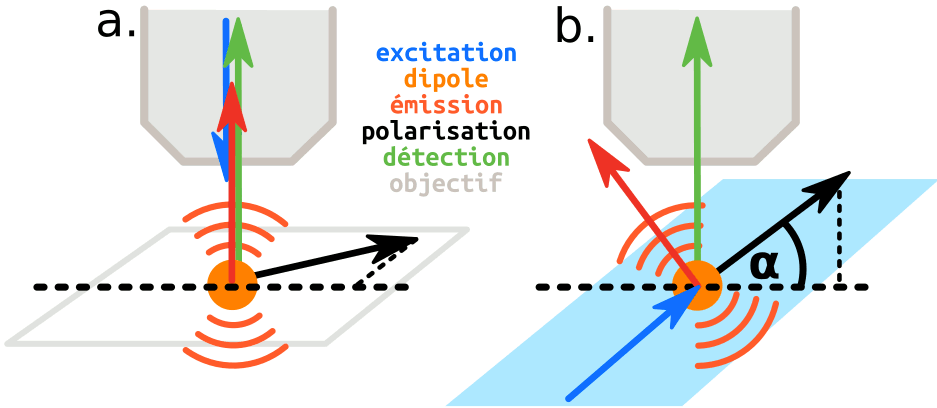
\includegraphics[width=0.8\textwidth]{./files/polarization_plane.svg.png}
\caption{a. Comme dans un microscope deux photons classique, la direction d'émission et de détection sont alignées, et la polarisation est dans le plan orthogonal. Quelle que soit la polarisation, la lumière détectée est toujours la même.
\\ b. Dans un microscope à feuille de lumière, la direction d'émission est dans le plan orthogonal à la détection. La direction de polarisation fait alors un angle $\alpha$ avec la direction de détection. Pour $\alpha$ = 90°, la lumière détectée est maximale, mais pour $\alpha$ = 0°, elle est nulle.}
\end{figure}


Il est donc important de caractériser le comportement de la fibre par rapport à la polarisation. Deux cas sont donc à envisager : une rotation de la polarisation et un changement d'ellipticité. En mesurant l'orientation de la polarisation en sortie de fibre, j'ai montré que celle-ci pouvait tourner largement en fonction de la courbure de la fibre. Par exemple, entre un rayon de courbure de 15 cm et 25 cm, une polarisation linéaire peut tourner de 10°. À cause de l'anisotropie du rayonnement dipôlaire, une polarisation tournée de 90° fait chuter le signal de 100\%. Une rotation de 10° fait chuter le signal de 17\%. En pratique, il est difficile de mainenir la fibre parfaitement droite, et donc de minimiser la rotation de la polarisation, c'est pourquoi j'ai cherché à obtenir une polarisation invariante par rotation, c'est-à-dire une polarisation circulaire.

% TODOVolker (real condition curvature)
% Again what is the expected curvature variation in your experimental configuration. What is the expected signal variation.
% préciser les courbures

En polarisation circulaire, la rotation n'est plus un problème, mais la fibre peut toujours transformer la polarisation circulaire en une polarisation elliptique, qui perd sa symétrie et devient donc sensible à la rotation. J'ai donc caractérisé la variation d'ellipticité dans le cas d'une polarisation circulaire. Pour cela, j'ai positionné deux puissance-mètre sur les bras d'un cube polariseur en sortie de fibre. Pour chaque courbure de fibre, je mesurais l'intensité minimale et l'intensité orthogonale, ce qui permet de déduire le grand axe (a) et le petit axe (b) de l'ellipse, et donc l'ellipticité ($\theta$) définie par

$$
\tan(\theta)=\frac{b}{a} 
$$

Je montre que l'ellipticité peut varier de 5° entre deux courbures extrêmes. Pour une polarisation elliptique à 40°, la différence entre grand axe et petit axe est de 16\%. Une rotation de 90° en polarisation elliptique avec cette ellipticité donnerait alors lieu à une variation de détection de 16\%, ce qui est beaucoup mieux que 100\%. Il est cependant nécessaire d'effectuer des tests en conditions réelles afin de vérifier que ce pire cas n'est pas atteint.

\subsubsection{Test en conditions réelles}

Pour tester les variations d'intensité dues aux déformations de la fibre en conditions réelles, j'ai monté un cube polariseur et un puissance-mètre à la place de l'échantillon et ai soumis l'ensemble à des stimulations périodiques guidées par un moteur.

\begin{figure}
\centering
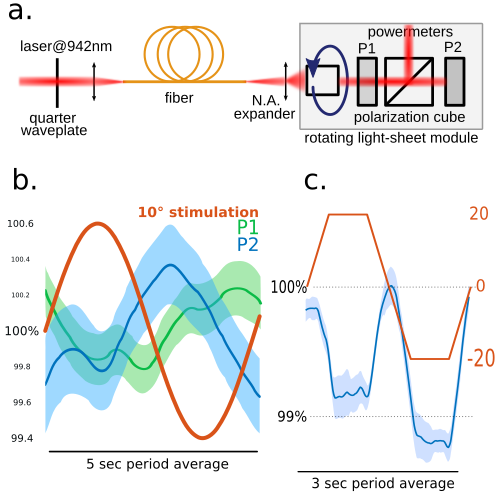
\includegraphics[width=0.8\textwidth]{./files/real-condition_intensity-variation.png}
\caption{
\\ a. Setup de test en condition réelle
\\ b. Réponse à une stimulation sinusoïdale périodique de 10°. On constate que les variations de puissance ne dépassent pas 0.6\% et que ces variations combinées aux changement de la polarisation (ellipticité et rotation) n'excèdent pas 1.2\%.
\\ c. Réponse à une stimulation périodique en marches de 20°. Les variations combinées n'excèdent pas 1.2\%. On remarque que l'intensité maximale est atteinte pour un angle du moteur de 0°, soit la position de repos de la fibre.
}
\end{figure}

Finalement, tous les effets liés à la position de la fibre engendrent des variations de l'intensité détectée inférieurs à 1.2\% dans les conditions des expériences. Les effets parasites sont donc connus et mineurs, ce qui est à prendre en compte lors de l'analyse des données.

% TODOVolker (intensity change due to polarization)
% You have also to add the measured intensity change in the case if you would work with linear polarized light. In addition you have to make a measurement with GFP fish to see how much the real collected fluorescence depends on polarization and ellipticity.

\section{Effet de lentille thermique}

% VolkerComment (introduce thermal lens effect)
% You need to introduce better this part. In the previous sections you characterized hollow core fibers and identified a fiber that fulfills the stringent requirements to build a fiber coupled 2P-RLS. You should finish this part with the demonstration of successful 2P whole-brain imaging with single cell resolution in static mode. Then you discuss the next challenge to record during dynamic microscope rotation. The challenge arises as you observed large intensity fluctuations during microscope rotation that are independent of fiber properties. Then you discuss that this instability is related to water movements as you can induce it by moving the water in the chamber while keeping the microscope static. You discovered that this instability results from a thermal lens effect ....
% [rephrased]
% - demonstrate static 2P fiber coupled imaging
% - then discuss the dynamic mode challenges

Un des problèmes auxquels j'ai été confronté est l'effet de lentille thermique (thermal lens effect). Lorsqu'un faisceau traverse un milieu absorbant, ce milieu chauffe sur la trajectoire du faisceau, ce qui change son indice optique. Le gradient d'indice ainsi formé dévie les rayons, formant une lentille à gradient d'indice (GRIN lens). Pour l'eau, à 915 nm, le changement d'indice est de l'ordre de -1e-4 par degré. La température étant plus élevée au centre du faisceau, l'indice optique est plus faible, et donc la lentille équivalente est divergente. Cet effet peut être utile, par exemple pour mesurer le coefficient d'absorption d'un liquide \cite{whinnery_laser_1974}, mais il a deux conséquences gênantes dans mon cas. D'une part un effet statique lié à la perte de focalisation du faisceau altère l'effet deux-photons, d'autre part un effet dynamique lié à la réponse du système à une perturbation de la température d'équilibre dévie le faisceau lors des mouvements du microscope.

% -1e-4 par degré
% https://en.wikipedia.org/wiki/Optical_properties_of_water_and_ice


\subsection{Effet statique}

% TODOVolker (thermal lens effect)
%  Explain this paper more in detail and show the schematic that explains the calculations and the approximation.

Le phénomène et a été décrit théoriquement en 1965 par Gordon \emph{et al} \cite{gordon_longtransient_1965} et en 1974 par Whinnery \emph{et al} \cite{whinnery_laser_1974} pour une fine cellule de liquide et dans le cadre de l'approximation parabolique. En 1982, Sheldon \emph{et al} \cite{sheldon_laser-induced_1982} étend cette description hors de l'approximation parabolique pour prendre en compte les aberration induites. Dans notre cas, il ne s'agit pas d'une cellule fine, car le laser traverse plusieurs centimètres d'eau avant d'atteindre l'échantillon, créant un gradient d'indice sur sa trajectoire. Je suis donc allé m'inspirer du livre *Gradient-Index Optics* (2002) \cite{gomez-reino_gradient-index_2002}, dans lequel les auteurs s'intéressent à la propagation d'un faisceau dans un milieu d'indice : (équation 1.63 du livre)

$$
n(r,z) = n_0(z) \left( 1 \pm \frac{g^2(z)}{2}r^2\right)
$$

Dans le cas d'un signe négatif (lentille convergente), les calculs sont largement détaillés et aboutissent à une solution oscillante. Malheureusement le cas d'un signe positif (lentille divergente) n'est pas exploré. Pour obtenir un résultat en ordre de grandeur, nous avons donc opté pour un approche discrète numérique en appliquant à chaque tranche de liquide d'épaisseur *l* les résultats obtenus pour une cellule fine \cite{gordon_longtransient_1965}\cite{whinnery_laser_1974}. Cette approximation ignore la diffusion thermique le long de l'axe et considère l'absorption négligeable.

Le différentiel de température par rapport à l'équilibre $\Delta T(r,t)$ est décrit par l'équation de diffusion :

$$
c\rho\frac{\partial}{\partial t}[\Delta T(r,t)] = \dot{q}(r) + k \nabla^2[\Delta T(r,t)]
$$

Le terme source de l'équation lié à l'absorption du faisceau de puissance *P* par le milieu de coefficient d'absorption $\alpha$ vaut :

$$
\dot{q}(r) = \frac{\alpha P}{\pi w^2_z}\exp \left(\frac{-2r^2}{w^2_z} \right)
$$

Ce qui donne une solution de la forme :

$$
\Delta T(r,t) = \frac{\alpha P}{4\pi k} \int_0^t \left( \frac{1}{1+2t'/t_c} \right) \exp \left( \frac{-2r^2/w_z^2}{1+2t'/t_c} \right) \mathrm{d}t'
\\
\text{où} \ t_c = \frac{w_z^2}{4D}
$$

Dans notre cas, on se contentera de l'approximation au premier ordre de cette solution :

$$
\Delta T(r,t) \simeq \frac{\alpha P}{4\pi k} \left[ \ln\left( 1+\frac{2t}{t_c} \right) - \frac{2(r^2/w_z^2)}{1+t_c/2t} \right]
$$

Le premier terme est indépendant de *r* et correspond au réchauffement progressif global de la tranche de liquide. De plus, il est de plus en plus lent à mesure que l'on s'éloigne du waist et se retrouve dominé par les conditions aux limites et par la diffusion le long de l'axe ici non exprimées. On peut donc l'ignorer pour simplifier le calcul sans altérer le résultat. On a donc :

$$
\Delta T(r,t) = \Delta T_\infty \frac{1}{1+t_c/2t}
\\
\text{où} \ \Delta T_\infty = \Delta T(r,t_\infty) = -\frac{\alpha P}{2\pi k}\frac{r^2}{w_z^2}
$$


Si l'on suppose constant le coefficient de variation de l'indice optique (*dn/dT*), on a donc un profil d'indice quadratique en *r* :

$$
n(r,z) = n_0 + \frac{\mathrm{d}n}{\mathrm{d}T}\Delta T
\\
n(r,z) = n_0 \left( 1+ \delta (r/w_z)^2 \right)
\\
\text{où} \ \delta = - \frac{\mathrm{d}n}{\mathrm{d}T} \frac{\alpha P}{2\pi kn_0} \frac{2}{1+t_c/2t}
$$

Pour un profil d'indice quadratique tel que celui-ci et dans l'approximation des lentilles minces, on peut définir la distance focale équivalente :

$$
f' = -\frac{w^2_z}{2ln_0\delta}
$$

Cela permet d'établir la valeur de la focale *F* au cours du temps :

$$
f'(t) = f'_\infty \left( 1 + \frac{t_c}{2t} \right)
\\
\text{où} \ f'_\infty = \frac{\pi k w_z^2}{\alpha Pl(\mathrm{d}n/\mathrm{d}T)}
$$

On part du principe que le faisceau reste gaussien tout au long du parcours, il peut donc être entièrement décrit pour chaque *z* par la position et la largeur de son waist. Pour chaque tranche de liquide d'épaisseur l, on peut donc écrire la formule des lentilles gaussiennes pour trouver le déplacement du waist et son élargissement.

\begin{figure}
\centering
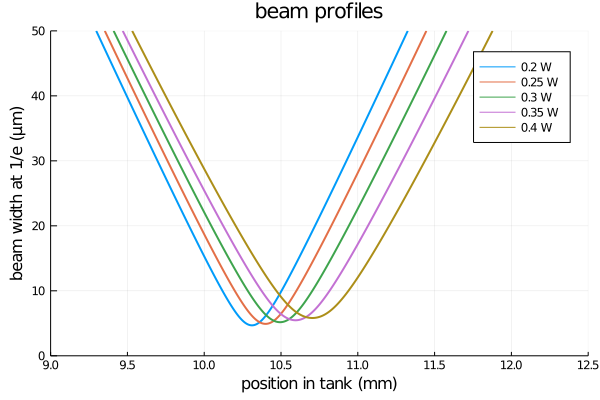
\includegraphics[width=0.8\textwidth]{./files/grinlensplots_profile.png}
\caption{
On voit ici le résultat de la simulation pour plusieurs puissances de laser. Comme attendu, plus la puissance est élevée, plus l'effet divergent est fort, et donc plus le waist est éloigné et large.
}
\end{figure}

On peut mesurer expérimentalement la position de cette largeur minimum du faisceau dans la fluorescine.

\begin{figure}
\centering
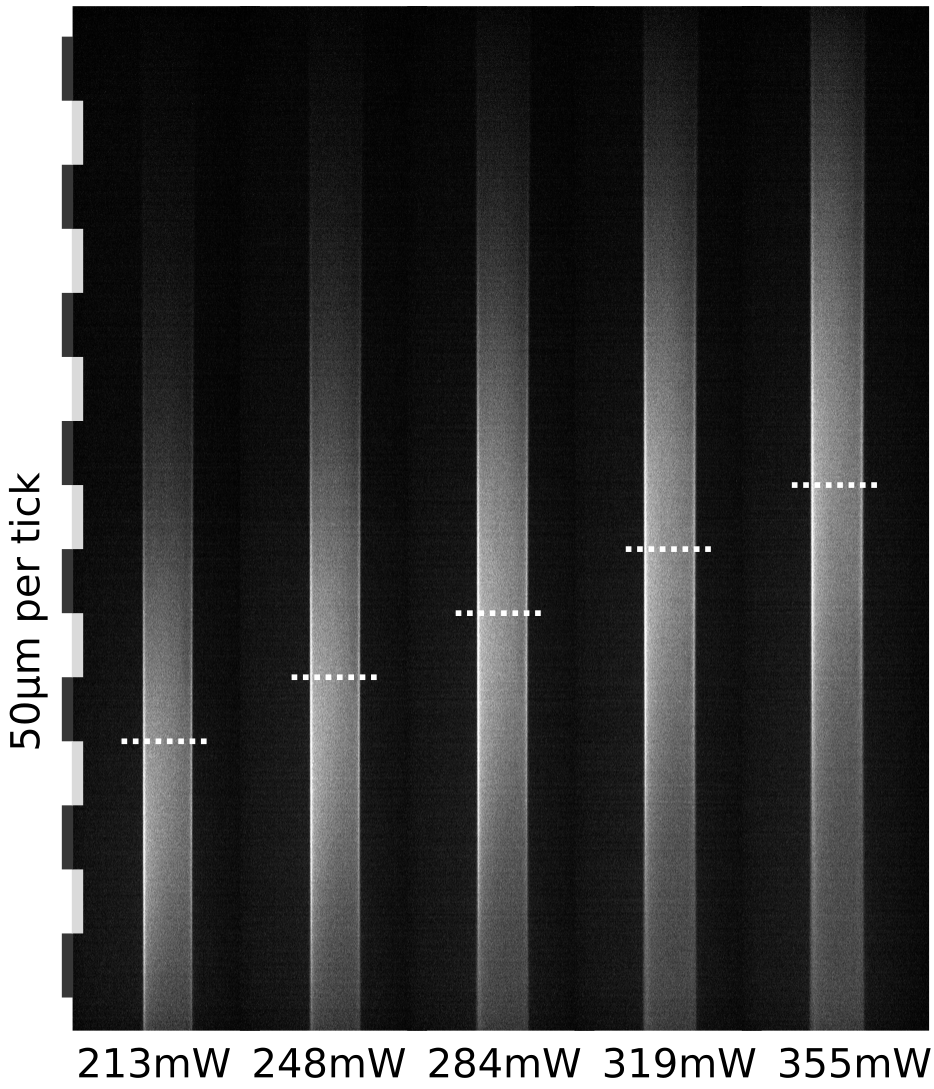
\includegraphics[width=0.8\textwidth]{./files/thermal-shift.svg.png}
\caption{
On voit ici une feuille de lumière imagée dans la fluorescéine pour plusieurs puissances laser différentes. La position du maximum d'intensité, et donc de la largeur minimale, est marquée par un trait en pointillé
}
\end{figure}

\begin{figure}
\centering
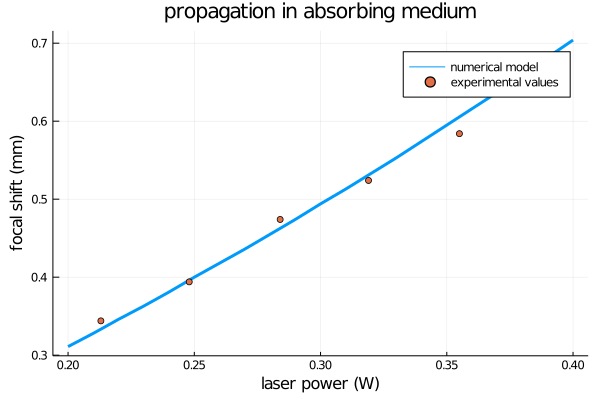
\includegraphics[width=0.8\textwidth]{./files/grinlensplots_model.png}
\caption{
voici la comparaison entre les données numériques et expérimentales
}
\end{figure}


\subsection{TODO analyse temporelle}